\chapter{BUILDING THE VARIOUS CLASSIFIERS}
The major idea behind this project is to build different classification models for the PIMA Indian Diabetes dataset, and to compare these models based on various evaluation parameters like accuracy, sensitivity, specificity, precision and error rate. In this regard, we intend to classify the data using decision tree algorithms like ID3, CART, C4.5 and ANN.
In the upcoming subchapters, the algorithmic aspect of these classifiers will be detailed.

\section{Decision Trees}
A decision tree is a decision support tool that uses a tree-like graph or model of decisions and their possible consequences, including chance event outcomes, resource costs, and utility. It is a flowchart-like structure in which each internal node represents a test on an attribute, each branch represents the outcome of the test, and each leaf node represents a class label (decision taken after computing all attributes). The paths from root to leaf represent classification rules.

A decision tree consists of three types of nodes:
\begin{enumerate}
    \item \textbf{Decision nodes} – typically represented by squares
    \item \textbf{Chance nodes} – typically represented by circles
    \item \textbf{End nodes} – typically represented by triangles
\end{enumerate}

The pseudo code of decision tree is followed as:-

\begin{figure}[h]
%\vspace{-3.8in}
\centering %\offinterlineskip
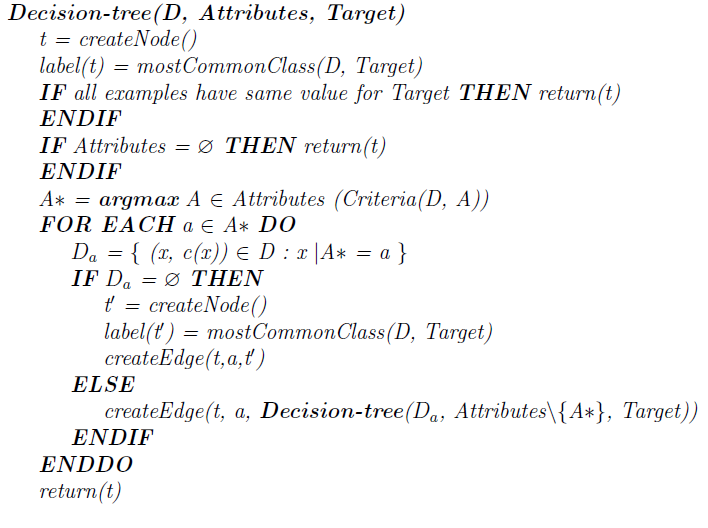
\includegraphics[scale=0.97]{dtcode.png}
\end{figure}
\pagebreak

The function \textbf{Criteria()} is the one that distinguishes the decision tree algorithms from each other. For all the models of decision tree, a 80-20 split was done on the dataset for training and testing the built model.

\subsection{ID3}
\begin{itemize}
    \item Select the attribute with the highest information gain.
    \item Let $p_i$ be the probability that an arbitrary tuple in $D$ belongs to class $C_i$ estimated by $ |C_{i,D}| / |D| $
    
    \newpage
    
    
    \item Expected Information (entropy) needed to classify a tuple in $D$
  
    \[ Info(D) = -\sum_{i=1}^{m} p_i \hspace{0.3cm} log_2(p_i) \]
    
    \item Information needed, after using $A$ to split $D$ into $v$ partitions to classify $D$
    
    \[ Info_A(D) = \sum_{j=1}^{v} \hspace{0.15cm} (|D_j| / |D|)
    \hspace{0.12cm} X \hspace{0.12cm} Info(D_j) \]
    
    \item Information gained by branching on attribute $A$
    
    \[ Gain(A) = Info(D) \hspace{0.12cm} - \hspace{0.12cm} Info_A(D)      \]
    
\end{itemize}

Computing Information gain for continuous-value Attributes:
\begin{itemize}
    \item Let attribute $A$ be a continuous value attribute
    \item The best split point for $A$ must be determined:
    \begin{itemize}
        \item Sort the value of $A$ in increasing order
        \item Typically, the midpoint between each pair of adjacent values is   considered as a possible split point
        \item $ (a_i + a_{i+1}) / 2 $ is the midpoint between the values of $ a_i $ and $ a_{i+1} $
        \item The point with the minimum expected information requirement for $A$ is selected as the split-point for $A$
    \end{itemize}
\end{itemize}
\newpage
Figure 4.1 visualizes the pruned version of our ID3 decision tree after training the model. It was constructed using mean for handling missing values. 
\vspace{0.27in}
\begin{figure}[h]
\centering 
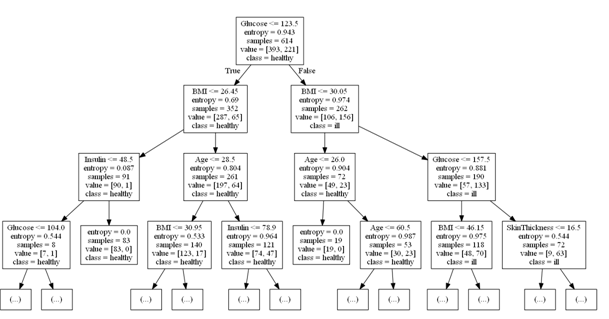
\includegraphics[width=7in,height=5in]{id3.PNG}
\caption{\label{fig:subBDDs1}ID3 decision tree}
\end{figure}
\newline
20\% of the dataset, i.e. 154 samples were used to validate the constructed decision tree. Figure 4.2 and 4.3 represents the output we obtained after building and testing our model.
\clearpage
\begin{figure}[h]
\centering
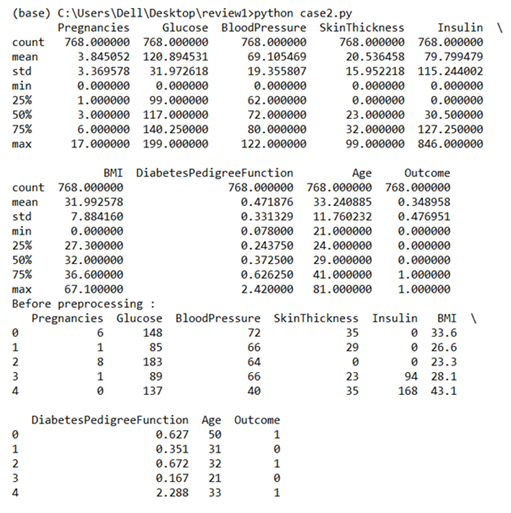
\includegraphics[scale=1.2]{sumbfprp.PNG}
\caption{\label{fig:subBDDs1}Summary of dataset before preprocessing}
\end{figure}
\pagebreak
\clearpage
\pagebreak
\begin{figure}[h]
\centering 
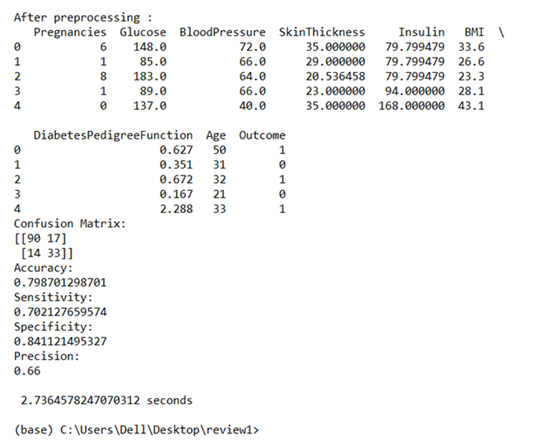
\includegraphics[scale=1.2]{dsfprp.PNG}
\caption{\label{fig:subBDDs1}Dataset after pre-processing and evaluation metrics}
\end{figure}
\pagebreak
\clearpage
\subsection{C4.5}
C4.5 (a successor of ID3) uses gain ratio to overcome the problem (normalization to information gain)
\[SplitInfo_A(D) = -\sum_{j=1}^{v} \frac{|D_j|}{|D|}\hspace{0.12cm} X \hspace{0.12cm}log_2(\frac{|D_j|}{|D|}) \]
\[GainRatio(A) = Gain(A)/SplitInfo(A)\]
\par \noindent
The attribute with the largest GainRatio is selected as the Splitting  Attribute.
For, J48 (Quinlan C4.5) to be implemented, attributes need to be categorized prior to training the model. So, we referred the method proposed in study [2] to categorize the dataset variables. The Table 4.1 summarizes the splitting criteria used for discretizing each attribute.
\begin{table}[h]
\begin{center}
\begin{tabular}{| c | c |}
  \hline
  \textbf{Attribute} & \textbf{Split Criteria} \\[0.85ex]
  \hline
  Pregnant & low(0,1), medium(2,3,4,5), high($>$6) \\[0.85ex]
  \hline
  Glucose & low($<$95), medium(95-140), high($>$140) \\[0.85ex]
  \hline
  Blood Pressure & normal($<$80), normal-high(80-90), high($>$90) \\[0.85ex]
  \hline
  BMI & low($<$24.9), normal(25-29.9), obese(30-34.9), severely-obese($>$35) \\[0.85ex]
  \hline
  DPF & low($<$0.5275), high($>$0.5275) \\[0.85ex]
  \hline
  Age & range-1($<$28.5), range-2($>$28.5) \\[0.85ex]
  \hline
\end{tabular}
\end{center}
\caption{\label{table:TT}Criteria for categorizing attributes in dataset}
\end{table}
\par \noindent
Since study [2] deleted 2 attributes namely, Skin Thickness and Insulin, the discretization for these two variables, was done using qcut function.  It is a Quantile-based discretization function provided by the Pandas library in Python.\par \noindent
Figure 4.4 visualizes the C4.5 decision tree constructed after categorizing the attributes in the Pima dataset using mean for handling missing values.
\begin{figure}[h]
\centering
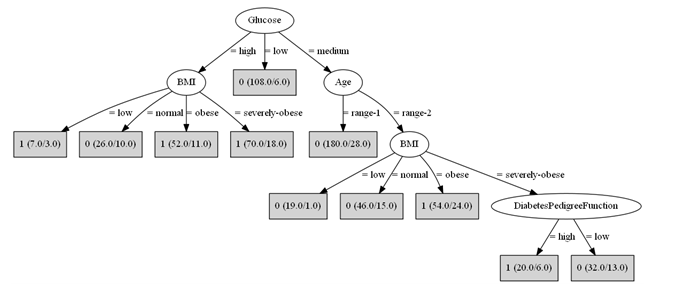
\includegraphics[scale=1.0]{c45.PNG}
\caption{\label{fig:subBDDs1}C4.5 Decision tree}
\end{figure}
\par \noindent
\newline 
20\% of the dataset, i.e. 154 samples were used to validate the constructed decision tree. Figure 4.5 represents the output we obtained after building and testing our model.
\begin{figure}[h]
\centering
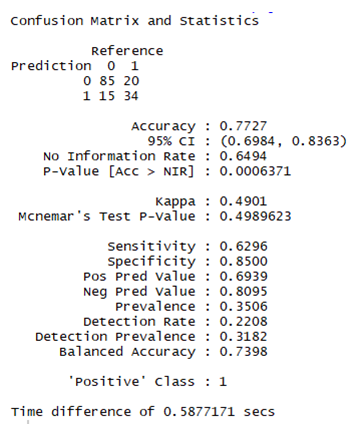
\includegraphics[scale=1.0]{c45eval.PNG}
\caption{\label{fig:subBDDs1}C4.5 evaluation metrics}
\end{figure}
\pagebreak



\subsection{CART}
\begin{itemize}
    \item If a data set D contains examples from n classes, gini index is defined as:
    \[ gini(D) = 1 - \sum_{j=1}^{n} p_j^2    \]
    \item If a data set D is split on A into two subsets D1 and D2, the gini index is defined as:
    \[ gini_A(D) = (|D_1| / |D|)gini(D_1) \hspace{0.12cm} + \hspace{0.12cm} (|D_2| / |D|)gini(D_2)    \]
    \item Reduction in Impurity:
    \[ \Delta gini(A) = gini(D) \hspace{0.12cm} - \hspace{0.12cm} gini_A(D) \]
    \item The attribute that provides the smallest $ginisplit(D)$ (or the largest reduction in impurity) is chosen to split the node.
    \item This is enumerated for all the possible splitting points for each attribute.
\end{itemize}
The Figure 4.6 visualizes the pruned version of our CART decision tree.
\begin{figure}[h]
\centering
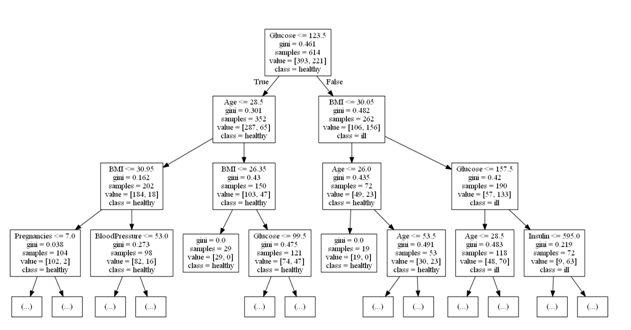
\includegraphics[width=7in,height=5in]{cart.PNG}
\caption{\label{fig:subBDDs1}CART Decision tree}
\end{figure}
\newpage
20\% of the dataset, i.e. 154 samples were used to validate the constructed decision tree. Figure 4.7 represents the output we obtained after building and testing our model.
\begin{figure}[h]
\centering
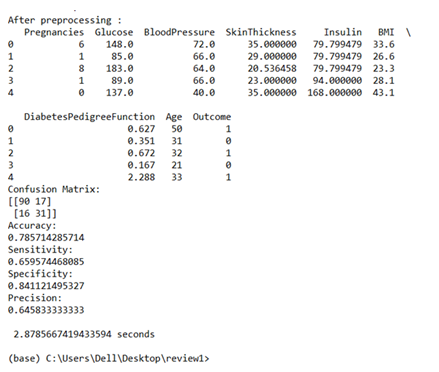
\includegraphics[scale=1.4]{carteval.PNG}
\caption{\label{fig:subBDDs1}CART evaluation metrics}
\end{figure}

\newpage
\section{ANN Algorithm}
Artificial Neural Networks are a computational tool modelled on the interconnection of the neuron in the nervous systems of the human brain and that of other organisms. They are composed of multiple nodes, which imitate biological neurons of human brain. The neurons are connected by links and they interact with each other. The nodes can take input data and perform simple operations on the data. The result of these operations is passed to other neurons. The output at each node is called its activation or node value. Each link is associated with weight. ANNs are capable of learning, which takes place by altering weight values.
\begin{figure}[h]
\centering
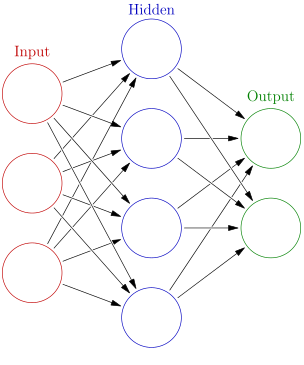
\includegraphics[scale=1.0]{ann.png}
\caption{\label{fig:subBDDs1}Struture of ANN}
\end{figure}
\par \noindent
There are two Artificial Neural Network topologies –
\begin{itemize}
\item \textbf{FeedForward ANN} - The information flow is unidirectional. A unit sends information to other unit from which it does not receive any information. There are no feedback loops.
\item \textbf{FeedBack ANN} - where, feedback loops are allowed.
\end{itemize}
\par \noindent
The ANN model that we have built for our data set has the following characteristics.
\begin{itemize}
\item We have built a feed-forward ANN with backpropagation.
\item One input layer, one hidden layer, and one output layer, each consisting of 12, 8, and 1 node(s) respectively. For convenience, from now on, we will refer to the input, hidden and output layers as i, h, and the o layers respectively.
\item The i, h, and the o layers use relu, relu, and sigmoid as their activation functions respectively.
\item Adam was used as the model optimizer.
\item Adam was used as the model optimizer.
\item The number of epochs ( the number of times for which the model sees the entire of the training data set ) was fixed to 1000.
\item The number of tuples per training batch ( batch size ) was fixed to 16.
\par \noindent
The impact of batch size was extensively studied by subjecting our Neural Network to various batch size values. The batch sizes considered are powers of 2 because of the efficient allocation of batches of dataset to the processors(or cores) in the system. The line chart built in Figure 4.9 summarizes the same.
\begin{figure}[h]
\centering
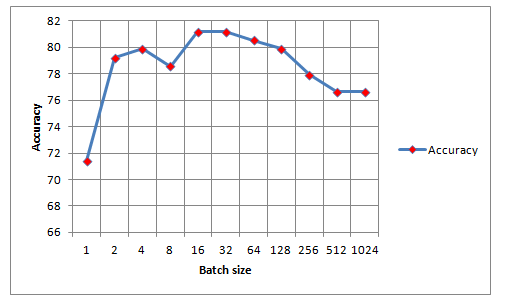
\includegraphics[scale=1.0]{batch.PNG}
\caption{\label{fig:subBDDs1}Impact of batch size}
\end{figure}
\pagebreak
From Figure 4.9, it’s clear that accuracy of ANN reaches its peak batch size of 16 and 32. Any value of batch size lower or higher gradually decreases the accuracy. Hence, our choice of 16 as batch size is well warranted for the constructed ANN.
\item 80\% of the entire dataset was used to train the model, and the rest was used to test the model.
\end{itemize}
\par \noindent
\newline
20\% of the dataset, i.e. 154 samples were used to validate the constructed decision tree. Figure 4.10 represents the output we obtained after building and testing our model.
\begin{figure}[h]
\centering
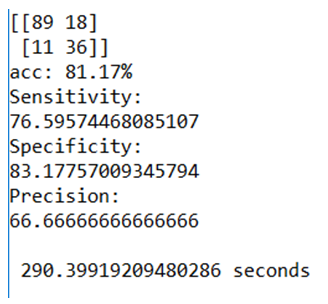
\includegraphics[scale=1.0]{anneval.PNG}
\caption{\label{fig:subBDDs1}ANN evaluation metrics}
\end{figure}
\pagebreak
\newline

\section{Evaluation Metrics}
Before training the models, the data set was randomly split into training and testing set. 80\% of the input data was used for training and the remaining 20\% was used for testing. The models are built by learning from training set and the unknown test set is used for computing evaluation metrics to analyze the quality of the models built.

\begin{itemize}
    \item The \textbf{confusion matrix} captures the information regarding the actual and predicted target class labels from the test set. The general structure of a confusion matrix is represented in Figure 4.11
    \newpage
    \begin{figure}[h]
    \centering
    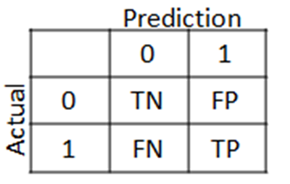
\includegraphics[scale=1.0]{cm.PNG}
    \caption{\label{fig:subBDDs1}Confusion Matrix}
    \end{figure}
    where,
    \begin{itemize}
        \item \textbf{TP} refers to the number of True Positive samples. They are test samples that are actually positive and classified as positive.
        \item \textbf{TN} refers to the number of True Negative samples. They are test samples that are actually negative and classified as negative
        \item \textbf{FP} refers to the number of False Positive samples. They are test samples that are actually negative but classified as positive
        \item \textbf{FN} refers to the number of False Negative samples. They are test samples that are actually positive but classified as negative
    \end{itemize}
\end{itemize}
Using the values from confusion matrix, the following evaluation metrics can be computed.
\begin{itemize}
    \item \textbf{Accuracy}: It is the ratio of number of samples correctly classified by the model and the total number of samples in the test set.
    \[
        Accuracy = \dfrac{TP+TN}{TP+TN+FP+FN}
    \]
    
    \item \textbf{Sensitivity}: It is the ratio of number of True Positive (TP) samples and the total number of positive samples in the test set.
    \[
        Sensitivity = \dfrac{TP}{TP+FN}
    \]
    
    \item \textbf{Specificity}:  It is the ratio of number of True Negative (TN) samples and the total number of negative samples in the test set.
    \[
        Specificity = \dfrac{TN}{TN+FP}
    \]
    \item \textbf{Precision}:  It is the ratio of number of True Positive (TP) samples and the total number of samples predicted as positive by the model.
    \[
        Precision = \dfrac{TP}{TP+FP}
    \]
\end{itemize}